\documentclass{jors}
\usepackage[utf8]{inputenx}
\usepackage{cmap}
\usepackage[T1]{fontenc}
\usepackage{textcomp}
\usepackage[english]{babel}
\usepackage[top=2cm,bottom=2cm,outer=2.2cm,inner=2.2cm]{geometry}
\usepackage[backend=biber,sortcites=true,doi=true,url=true,firstinits=true,hyperref,maxbibnames=9,maxcitenames=3,sorting=nyt]{biblatex}

\addbibresource{refs.bib}
\usepackage{csquotes}
\usepackage{url}
\usepackage{hyperref}
\usepackage{mathtools}
\usepackage{dsfont}

\usepackage{userdefs}

\begin{document}

\twocolumn[
  \begin{@twocolumnfalse}
    \begin{minipage}{0.3\textwidth}
      \rule{100pt}{12pt} % Logo placeholder
    \end{minipage}
    \begin{minipage}{0.65\textwidth}
      \scriptsize
      \authorshort \ \pubyear \ \mytitle. Journal of Open Research Software,
      \pubnumber: \pubed, DOI: \url{\pubdoi}
    \end{minipage}
    \twrule
    \begin{flushleft}
      {\bf \large SOFTWARE METAPAPER} \vspace{9pt} \\
      {\bf \LARGE \mytitle } \\ \vspace{0.2cm}
      {\large \myauthor} \\ \vspace{0.2cm}
      {\footnotesize \myaffiliation}
    \end{flushleft}
    \twrule
    \begin{abstract}
      A very important part of research in Mathematical Optimization field is to benchmark
optimization packages because it is one of the ways to compare
solvers.
During benchmarking, one usually
obtains a large amount of information, like CPU time, number of functions
evaluations, number of iterations and much more. This information, if
presented as tables, can be difficult to be analyzed and compared, due, for instance, to
large amount of data.  Therefore, 
tools to better process and understand optimization benchmark data  started to be developed and tested. One of
the most widespread tools  is the \emph{Performance Profile} graphics proposed by
\textcite{Dolan:2002du}. In this context, this paper describes  perprof-py, a free/open source software
that makes Performance Profile graphics in a user-friendly manner. This software produces graphics in PDF using LaTeX with
PGF/TikZ~\cite{TikZ} and PGFPLOTS~\cite{pgfplots} packages, in
PNG using matplotlib~\cite{Hunter:2007}, and in HTML using
Bokeh~\cite{url:bokeh}. Perprof-py  can also be easily
extended to be used with other plot libraries,  it is implemented
in Python 3 with support for internationalization, and is under the General
Public License Version 3 (GPLv3).

    \end{abstract}
    \twrule
    \begin{flushleft}
      {\bf Keywords: }{\mykeywords}
    \end{flushleft}
    \twrule
  \end{@twocolumnfalse}
]

\section{Overview}
\subsection*{Introduction}

    When creating a software, it is usual to evaluate it regarding a set of
    information of interest
    --- such as CPU time, number of
    functions evaluations, number of iterations, memory usage, accuracy, or
    others --- in a
    process called \emph{benchmarking}.

    Benchmarking is a necessity as it
    helps uncover deficiencies in the software and generally lead
    to software
    improvements~\cite{url:mittelmann,Mittelmann:1999fb,Dolan:2006kl}.
    Furthermore, given a set of softwares to solve the same problem, one could
    compare them to choose the best one, or verify how his own software can be
    improved.
    In this sense, \textcite{Dolan:2002du} developed a tool to compare
    optimization solvers benchmarks: the \emph{performance profile}.

    The performance profile is a tool to evaluate and compare the performance
    of a set $\Sset$ of solvers  on a given test set $\Pset$, with respect
    to a chosen evaluation parameter,
    which we will reference as \emph{cost}.
    It is presented as
    a graphic that shows the cumulative distribution function of different
    solvers performances, according to the chosen cost metric.
    It is noteworthy that the cost metric must be positive.

    This comparison method is mostly used for nonlinear optimization solvers,
    however, it is possible to extend the performance profile to compare
    softwares that solve any kind of problem.
    For instance, some authors have used it in the context of algorithms for
    matrix functions \cite{al-mohy:2009, al-mohy:2011, al-mohy:2012,
    higham:2005, higham:2009, higham:2011, higham:2013}.
    Notice that, in some cases, a
    specialized test can be more significant than the performance profile with
    a specific cost.  For derivative-free optimization, for instance,
    \textcite{More:2009benchmarking} define a \emph{data profile}, using the
    number of function evaluations as the metric cost, nevertheless in a 
    different way of performance profile definition.

    For each
    problem $p \in \Pset$ and solver $s \in \Sset$, let $t_{p,s}$ be the
    cost required to solve problem $p$ by solver $s$ and
    \begin{align*}
      r_{p,s} = \frac{t_{p,s}}{\min\{t_{p,s}: s \in \Sset\}}
    \end{align*}
    be the performance ratio of solver $s$ for the problem $p$ when compared
    with the best performance by any solver on this problem.
    As a convention, we set $r_{p,s}$ to a large value, let's say $r_{\max}$, if
    the solver $s$ does not solve the problem $p$.

    The probability of a solver $s \in \Sset$  to solve one problem within a
    factor $\tau \in \mathds{R}$ of the best performance ratio is the function
    \begin{align*}
      \rho_s(\tau) = \frac{| \{p \in \Pset: r_{p,s} \leq \tau\} |}{| \Pset |}.
    \end{align*}
    For a given $\tau$, the best solver is the one with the highest value for
    $\rho_s(\tau)$, that is, the one with the highest probability to solve the
    problem.
    The value $\rho_s(\tau)$ represents the percentage of problems solved by
    algorithm $s$ with a cost at most $\tau$ times worst than the best
    algorithm. $\rho_s(1)$ is the percentage of problems solved as fast as the
    fastest algorithm, which gives the efficiency of solver $s$.
    On the other hand
    \[\displaystyle \lim_{\tau\rightarrow r^-_{\max}} \rho_s(\tau)\]
    is the total percentage of problems solved by solver $s$, in
    other words, the robustness of solver $s$.

\subsection*{Motivation}

    To facilitate the reproduction of data set analysis, such as the
    benchmarking of solvers analysis provided by \textcite{Dolan:2002du}'s
    performance profile, it is important to have an open source tool that handle
    the production of plots.

    Performance profile has been, over the years, the most used benchmark
    comparison tool used in optimization. Nevertheless, the production of such
    analysis is sometimes a dull task, that can lead a researcher to waste a lot
    of time and effort that should have been spent in developing the solver
    itself.

    There are other
    implementations to generate  performance profiles,
    some of them being reasonable well-known, such as a MatLab
    script\cite{url:cops} from
    the same group that created the performance profile,
    and a module written by
    Michael Friedlander inside
    NLPy~\cite{url:NLPy}.

    Some, perhaps unaware of these implementations or avoiding
    proprietary solutions, made their own implementation and then made them
    available, such as a Python function perfprof from \textcite{url:perfprof} 
    and a small Julia module {\tt perfprof.jl} from \textcite{url:perfprofjl}, 
    both language dependent. A through search would possible reveal many
    others.
    However, there are features that some users need that those softwares have
    not implemented.

    In this work, it is described a straightforward open source tool that
    allows  one to create  performance profile pictures in a fast and easy
    manner.
    In addition, this tool  allows LaTeX users, a group in which almost
    all optimization community is included, to generate performance profile
    plots as LaTeX code that will be processed later  with the rest of their document or standalone PDF when needed.

    With these two main goals in mind,  perprof-py was developed and 
    implemented in Python 3 with internationalization features and direct LaTeX
    integration.

\subsection*{Implementation and architecture}

    The software was implemented as a Python 3 package
    and organized to allow addition of new backends.
    The core files are
    \begin{itemize}
      \item {\tt perprof/prof.py} that defines a class {\tt Pdata} that need to
        be extend for every backend;
      \item {\tt perprof/parse.py} that has the parser for the input files; and
      \item {\tt perprof/main.py} that has the command line interface.
    \end{itemize}

    The choice for perprof-py not be compatible with Python 2
    was due (i) the fact that unicode processing with Python 2 can be a nightmare and
    (ii) the authors desire to push Python 3 forward.

    Users have a command line interface to use out of the box,
    however one can also use the package in their own software.

    The implementation is very straightforward. The algorithm:
    \begin{enumerate}
      \item parses the options passed as arguments, creating a
        structure with all the information;
      \item parses and process the input files, using the definition
        of the performance function to create the data to be plotted;
      \item uses the chosen backend to plot the data.
    \end{enumerate}

\subsection*{Input}

    For each solver to be compared in the benchmark, one must write a file in
    the following manner:

    \begin{verbatim}
---
YAML information
---
Problem01 exit01 time01
Problem02 exit02 time02
    \end{verbatim}

    The YAML\cite{url:yaml,url:pyyaml} information is a list of keywords and values used to
    set the name of the solver and some
    flags for perprof-py.
    A legacy option remains in which the user can instead put only the
    solver name using
\begin{verbatim}
#Name SOLVERNAME
Problem01 exit01 time01
Problem02 exit02 time02
\end{verbatim}
    however it is possible that some users  will like to
    add more options.

    Each line of data has at least 3 columns.
    The columns' meaning, in a default order, are:
    \begin{itemize}
      \item The name of the problem;
      \item Exit flag;
      \item Cost measure -- for instance, elapsed time.
    \end{itemize}
    The default exit flag is to have {\tt c} or {\tt d} on the exit flag
    columns, meaning convergence or divergence, respectively.

    One of our example solvers uses the following YAML information
\begin{verbatim}
algname: Alpha
success: converged
free_format: True
\end{verbatim}
    which means that the name appearing on the profile will be {\tt Alpha};
    that {\tt converged} is the word that means convergence,
    and that every other exit flag word means divergence.
    These options were set from {\tt algname}, {\tt success} and {\tt
    free\_format} options, respectively.

    The user can, optionally, add more columns to give additional information.
    He can verify, for instance, that the optimality conditions are satisfied
    for each problem.
    Also, using  YAML or  command line options, the user can change the
    meaning of each columns.
    Notice that these options are not enabled by default. The user should
    consult the help and documentation to see how to enable them.

\subsection*{Parsing process and output}

    To use perprof-py, the user needs to issue a command of the type
\begin{verbatim}
$ perprof OPTIONS BACKEND FILES
\end{verbatim}
    where
    \begin{itemize}
      \item FILES are the input files described in the previous section. At
        least two files input are required;
      \item BACKEND is one of the options \verb+--tikz+, \verb+--mp+,
        \verb+--bokeh+ or
        \verb+--raw+, which represents whether the user wants to use
        TikZ/PGFPLOTS, matplotlib, Bokeh, or simply printing the performance
        ratios, respectively;
      \item OPTIONS are varied arguments that can be passed to perprof-py to
        customize the graphics or modify the performance functions. Some
        noteworthy options are
        \begin{itemize}
          \item \verb+--semilog+: the natural logarithmic scale is used on the
          abscissa axis;
          \item \verb+--success STR+: \verb+STR+ is a comma separated string
            of keys that was considered  \emph{success} by the solver;
          \item \verb+--black-and-white+: perprof-py creates the plots using
            only line styles and it colors them in black;
          \item \verb+--subset FILE+: perprof-py considers only the subset problems listed in \verb+FILE+, while creating the performance functions.
        \end{itemize}
    \end{itemize}
    In order to demonstrate such OPTIONS, Figures
    \ref{fig:example1}-\ref{fig:example4} show some examples of  performance
    profile graphics.
    Figure \ref{fig:example1} shows the performance profile graphic with default
    options. Note that the lines are clumped due to the maximum time allowed
    in the solver.
    \begin{figure}[!ht]
      \centering
      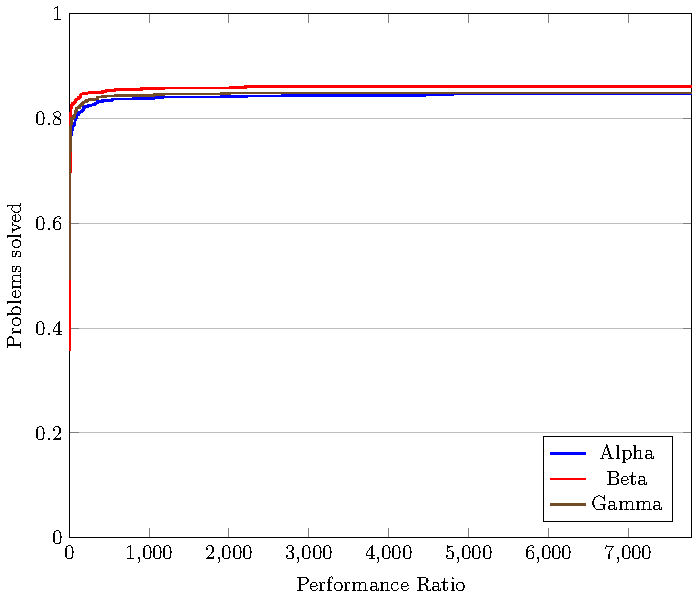
\includegraphics[width=0.4\textwidth]{plots/abc.pdf}
      \caption{Example of performance profile with default options.}
      \label{fig:example1}
    \end{figure}
    Figure \ref{fig:example2} shows the performance profile using the semilog
    option, which plots the graphic using a log scale on the abscissa.
    \begin{figure}[!ht]
      \centering
      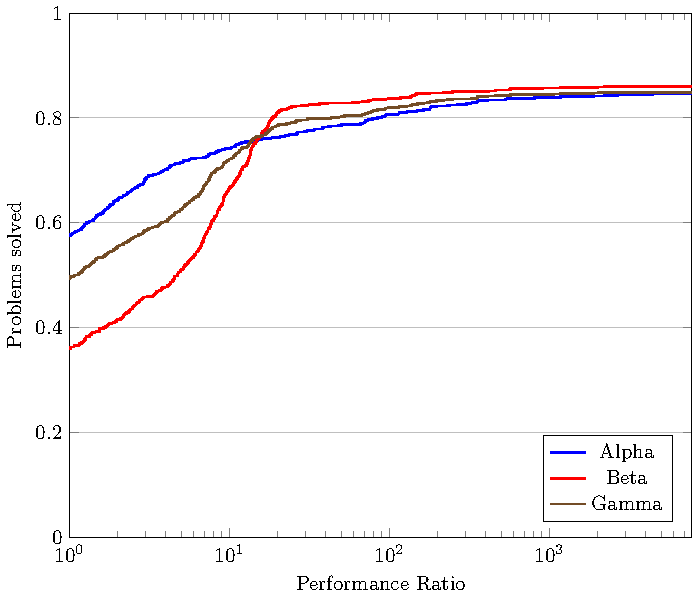
\includegraphics[width=0.4\textwidth]{plots/abc-semilog.pdf}
      \caption{Example of performance profile with semilog option.}
      \label{fig:example2}
    \end{figure}
    Figure \ref{fig:example3} shows the performance profile using also the black
    and white option, which gives a printer-friendly graphic.
    \begin{figure}[!ht]
      \centering
      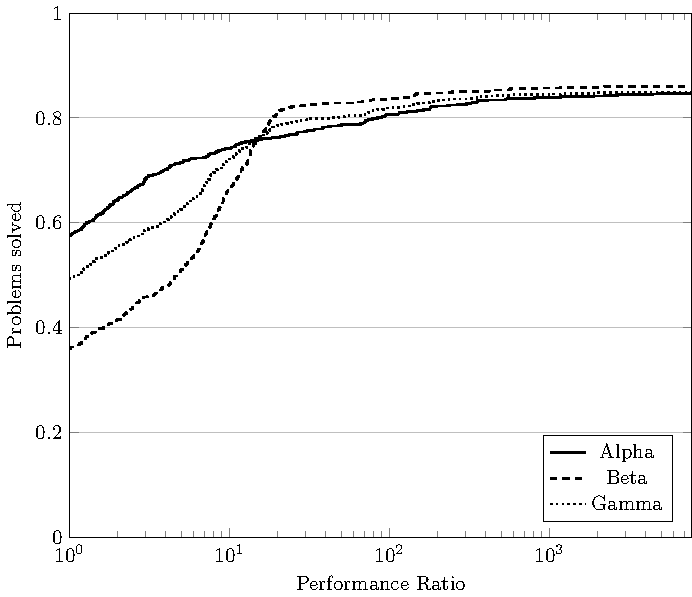
\includegraphics[width=0.4\textwidth]{plots/abc-semilog-bw.pdf}
      \caption{Example of performance profile with semilog and black and white
        options.}
      \label{fig:example3}
    \end{figure}
    Figure \ref{fig:example4} shows the performance profile using the subset
    option in addition to previous options. In this case, we selected around 120
    problems, put their names in a file, and passed the file with the option.
    This limits the comparison to only those files.
    \begin{figure}[!ht]
      \centering
      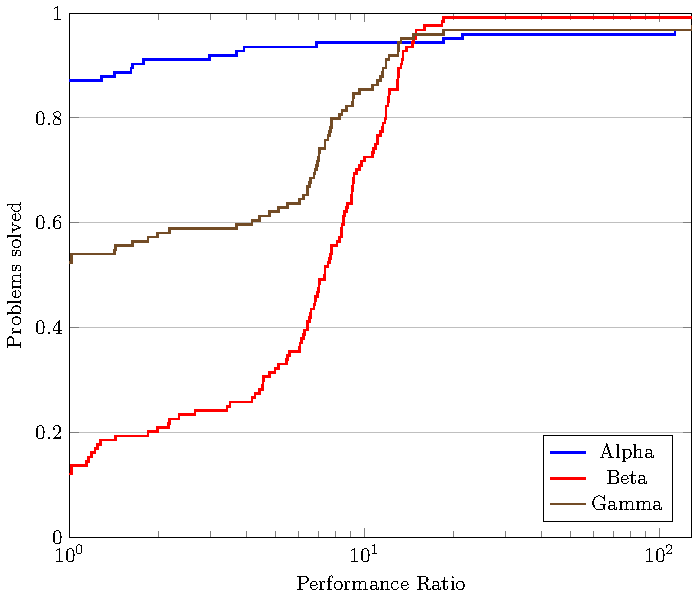
\includegraphics[width=0.4\textwidth]{plots/abc-semilog-hs.pdf}
      \caption{Example of performance profile with semilog and subset options.}
      \label{fig:example4}
    \end{figure}

\subsection*{Quality control}

    The code is tested using unit tests that verify if wrong input information
    is captured. These tests are run automatically on Travis CI
    \cite{url:travis}, for Python 3.3 and 3.4.
    In addition, also a script is run to generate several performance profile
    graphics. This script is also run on Travis CI, however the verification
    that perprof-py outputs the desired  graphics can be done only locally.

    This script uses artificial solver information accessible using \verb+--demo+
    as argument in the perprof-py call.
    For instance, to test that the TikZ installation is successful, one can run
\begin{verbatim}
perprof-py --demo -o tmp --tikz
\end{verbatim}
    If everything is correct, this will generate a file \verb+tmp.pdf+ with an
    example performance profile made using LaTeX and compiled to a standalone
    PDF.

    The user can run the testing script
    by entering the folder
    \verb+perprof/examples+ relative to the package folder, and running
\begin{verbatim}
./make-examples.sh
\end{verbatim}
    The folder \verb+plots+ will contain the outputs in formats PNG and PDF.


\section{Availability}
\subsection*{Operating system}

    Perprof-py is developed and actively tested on Unix platforms.
    The authors did not test it on Windows.

\subsection*{Programming language}

    The project was built entirely on Python 3.

\subsection*{Additional system requirements}

    No additional hardware requirement are necessary.

\subsection*{Dependencies}

    Perprof-py depends on the Python packages \texttt{matplotlib}, \texttt{pyyaml} and \texttt{bokeh}.
    In addition, if a user wants the PDF image from the LaTeX
    version, it also requires \texttt{pdflatex}.

\Archive

    \subsubsection*{Name:} perprof-py v1.1.0

    \subsubsection*{Identifier:} \url{\pubdoi}

    \subsubsection*{Licence:} GPL (General Public License) Version 3

    \subsubsection*{Date published:} 30/05/15

    \subsubsection*{Publisher:} Abel Soares Siqueira

    \subsubsection*{Date published:} 30/05/15

\CodeRepository

    \subsubsection*{Name:} GitHub

    \subsubsection*{Identifier:} \url{https://github.com/ufpr-opt/perprof-py}

    \subsubsection*{Licence:} GPL (General Public License) Version 3

    \subsubsection*{Date published:} 30/05/15

\subsubsection*{Language}

    The entire project was developed in English, but there is support for
    other languages on the code. Currently, the only other language implemented, besides English, is Brazilian Portuguese.



\section{Reuse potential}
Implementation is separated in a way that facilitates the creation of a
new backend.
Class {\tt Pdata} is defined to store the parsed data ($\mathcal{P}$,
$\mathcal{S}$, $t_{s,p}$, etc.) and  methods are defined to create the profile data
$r_{p,s}$.
Backends are classes that extend {\tt Pdata} defining a method {\tt plot}
which creates the expected figure.
One shall have little difficulty creating his own backend, specially if he
uses one of perprof-py own as a starting point.
However, if a user wants to change the profile data definition --- as
to implement  data profile (see \cite{bib:more2009benchmarking}) ---, he would have to modify
one or more methods in {\tt Pdata} directly or re-implement the backends.

Parser opens the input files and creates the information for {\tt Pdata}.
Replacing this parser --- to use with perprof-py backends --- would not be an easy task
since the correct output format should be created.  Nevertheless,
extending it with additional options would be simple enough.

Entry point {\tt perprof-py} essentially collects the options from the command
line and calls the specific backend profiler. This can be completely bypassed
by calling the backend directly. This allows one to create a performance
profile from another python application. In particular, one possibility is the
creation of a graphical user interface (GUI)
or a web server application. Perprof-py modularity 
allows whoever desires to construct this interface to focus entirely on
obtaining the options from the user and passing it to the backend.

Whether one is planning on expanding some of perprof-py functionalities or creating any
new backend or interface, he can contact the authors using the project page on
GitHub~\cite{url:perprof-py}.




\section*{\colorsectionnumberless{Acknowledgments}}
The authors would like to thank FAPESP\footnote{Grants 2008/09685-8 and 2009/17273-4.}
and CNPq\footnote{Grant 501763/2013-9.} for the
partial support given to this project
and their colleagues from LPOO and IMECC/UNICAMP.
In addition, the authors are grateful for the valuable insights and suggestions 
given by Miles Lubin and by the three anonymous reviewers, which improved
{\tt perprof-py} and this paper.

\printbibliography
\end{document}
